%%%%%%%%%%%%%%%%%%%%%%%%%%%%%%%%%%%%%%%%%%%%%%%%%%%%%%%%%%%%%%%%%%%%%%%%%%%%%%%%
\chapter{The Microarray Layout Problem}
\label{ch:mlp}
%%%%%%%%%%%%%%%%%%%%%%%%%%%%%%%%%%%%%%%%%%%%%%%%%%%%%%%%%%%%%%%%%%%%%%%%%%%%%%%%

In this chapter we give a more precise definition of the Microarray Layout
Problem (MLP) and define criteria for evaluating a given layout. The description
that follows assumes that synthesis is done by photolithographic masks, but the
concepts apply to the maskless production as well. Two evaluation criteria are
presented: \emph{border length} and \emph{conflict index}. As shown
later, the conflict index model can be seen as a generalization of the border
length model.

Formally, we have a set of probes $\mathcal{P} = \{p_{1}, p_{2},
\dots, p_{n}\}$ (frequently, but not necessarily, all probes have the
same length), where each $p_k \in \{\text{A,C,G,T}\}^\ast$ is
produced by a series of $T$ synthesis steps. Each step $t$ uses a mask
$M_t$ to induce the addition of a particular nucleotide $N_t \in
\{\text{A,C,G,T}\}$ to a subset of~$\mathcal{P}$
(Fig.~\ref{fig:masking_process}).  The \emph{nucleotide deposition
  sequence} $N = N_{1} N_{2} \ldots N_{T}$ corresponding to the
sequence of nucleotides added at each synthesis step is therefore a
supersequence of all $p \in \mathcal{P}$.

A microarray chip consists of a set of spots, or sites, $\mathcal{S} =
\{s_{1}, s_{2}, \dots, s_{m}\}$, where each spot $s$ is specified by its
coordinates on the chip surface and accommodates a unique probe
$p_k \in \mathcal{P}$. Note that we usually refer to $s$ as
containing a single probe $p_k$ although, in practice, it
contains several million copies of it. Each probe is synthesized at a
unique spot, hence there is a one-to-one assignment between probes and
spots (if we assume that there are as many spots as probes, i.e.,
$m=n$).

In general, a probe can be \emph{embedded} within $N$ in several ways.
An embedding of $p_{k}$ is a $T$-tuple $\eps_{k} = (\eps_{k,1},
\eps_{k,2}, \dots, \eps_{k,T})$ in which $\eps_{k,t} = 1$ if probe
$p_{k}$ receives nucleotide $N_{t}$ (at step~$t$), and 0 otherwise.  In
particular, a \emph{left-most embedding} is an embedding in which the
bases are added as early as possible (as in $\eps_1$ in
Fig.~\ref{fig:masking_process}).  We say that a spot or an embedding
$\eps_k$ is \emph{productive} (unmasked) at step $t$ if $\eps_{k,t} =
1$, or \emph{unproductive} (masked) otherwise.


\begin{figure}
\centerline{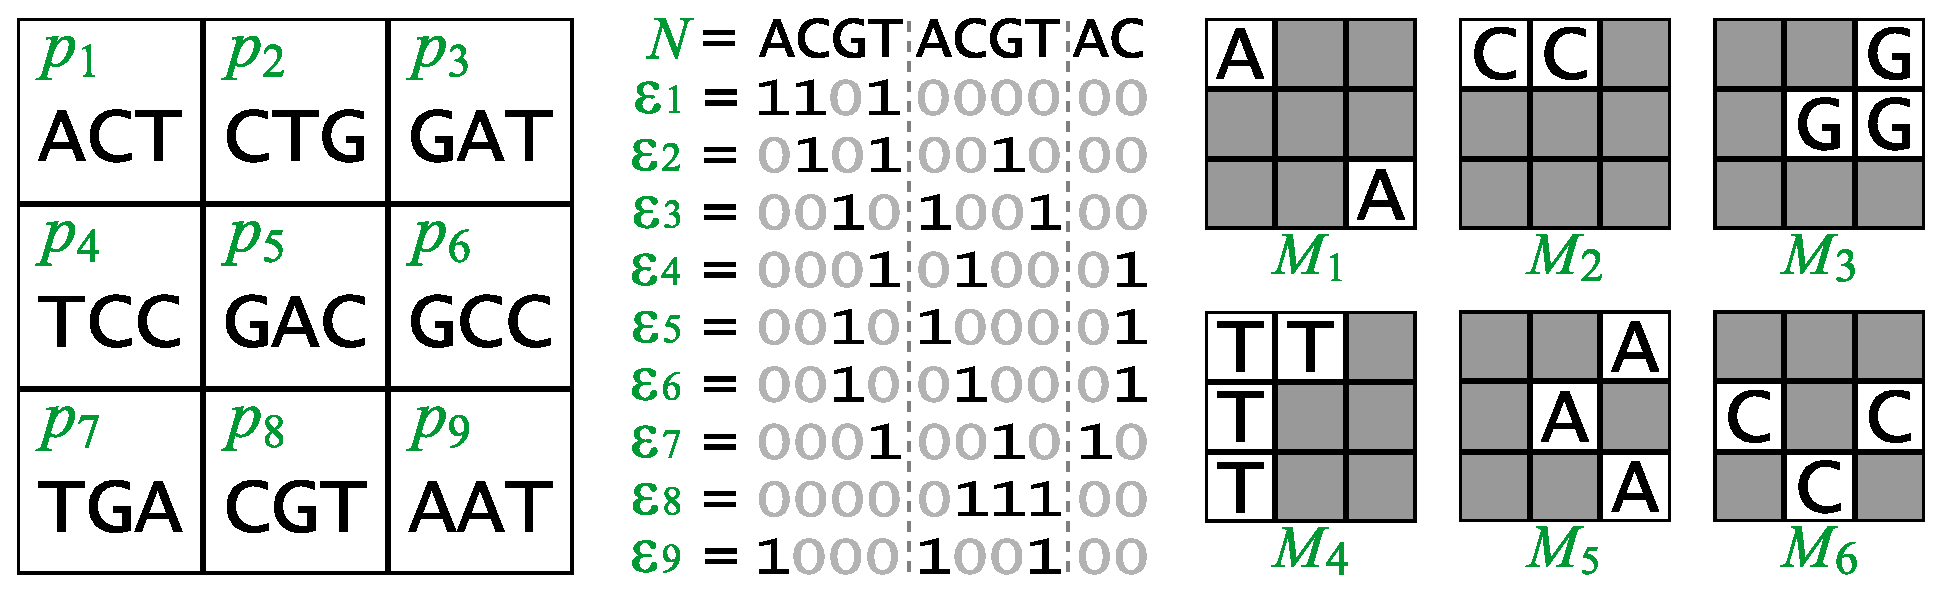
\includegraphics[width=\textwidth]{figures/chip.eps}}
\caption{Synthesis of a hypothetical 3$\times$3 chip with photolithographic
masks. Left: chip layout and the 3-mer probe sequences. Center: deposition
sequence and probe embeddings. Right: first four masks.}
\label{fig:masking_process}
\end{figure}

The deposition sequence is often a repeated permutation of the alphabet, mainly
because of its regular structure and because such sequences maximize the number
of distinct subsequences \citep{Chase1976}. The deposition sequence shown in
Fig.~\ref{fig:masking_process} is a 2.5-time repetition of ACGT, and we thus
say that it has two and a half \emph{cycles}.

For cyclic deposition sequences, it is possible to distinguish between two
types of embeddings: \emph{synchronous} and \emph{asynchronous}. In the first
case, each probe has exactly one nucleotide synthesized in every cycle of the
deposition sequence; hence, 25 cycles or 100 steps are needed to synthesize
probes of length 25. In the case of asynchronous embeddings, probes can have
any number of nucleotides synthesized in any given cycle, allowing shorter
deposition sequences. For this reason, asynchronous embeddings are usually the
choice for commercial microarrays.  For instance, all GeneChip arrays are
asynchronously synthesized in 74~steps (18.5 cycles of TGCA), so only
sub-sequences of this particular deposition sequence can be selected as probes
on Affymetrix chips.  \citet{Rahmann2006SubsequenceCombinatorics} shows that
this covers about 98.45\% of all 25-mers.

Ideally, the deposition sequence should be as short as possible in order to
reduce manufacturing time, cost and probability of errors \citep{Rahmann2003}.
Finding the shortest deposition sequence to synthesize a set of probes is an
instance of a classical computer science problem known as the Shortest Common
Supersequence problem. Here, however, we assume that $N$ is a fixed sequence
given as input.

\section{Problem statement}
\label{sec:mlp_problem}

Given a set of probes $\mathcal{P}$, a geometry of spots $\mathcal{S}$,
and a deposition sequence $N$ as specified above, the MLP asks to
specify a chip layout $(k,\eps)$ that consists of
\begin{enumerate}
\item a bijective assignment $k: \mathcal{S}\to \{1,\dots,n\}$ that
  specifies a probe index $k(s)$ for each spot $s$ (meaning that
  $p_{k(s)}$ will be synthesized at $s$),
\item an assignment $\eps: \{1,\dots,n\}\to \{0,1\}^T$ specifying an
  embedding $\eps_k = (\eps_{k,1},\dots,\eps_{k,T})$ for each
  probe index $k$, such that $N[\eps_k] :\equiv (N_t)_{t:
    \eps_{k,t}=1} = p_k$,
\end{enumerate}
such that a given penalty function is minimized.  We introduce two
such penalty functions: total border length and total conflict index.

%We may thus speak of $\eps_{k(s)}$ as the embedding at spot $s$.

\section{Border length}
\label{sec:mlp_border_length}

A precursor of the MLP (that did not consider different embeddings)
was formally stated by Hannenhalli and co-workers \citep{Hannenhalli2002},
who defined
the \emph{border length}~$\mathcal{B}_t$ of a mask~$M_{t}$ as the
number of borders separating masked and unmasked spots at synthesis
step~$t$, that is, the number of border
conflicts in $M_{t}$. The total border length of a given layout is the
sum of border lengths over all masks. For example, the four masks
shown in Fig.~\ref{fig:masking_process} have $\mathcal{B}_1 = 4$,
$\mathcal{B}_2 = 3$, $\mathcal{B}_3 = 5$ and $\mathcal{B}_4 = 4$. The
total border length of that layout is 52 (masks 5 to 10 not shown).

The total border length is a possible penalty function to evaluate a
proposed layout, and the \emph{Border Length Minimization Problem}
(BLP) is then defined as the problem of finding a layout minimizing
total border length.


\section{Conflict index}
\label{sec:mlp_conflict_index}

The border length measures the quality of an individual mask or set of masks.
With this model, however, it is not possible to know how the border conflicts
are distributed among the probes. Ideally, all probes should have roughly the
same risk of being damaged by unintended illumination, so that all signals are
affected by the resulting imperfections in approximately the same way.

The \emph{conflict index} is a quality measure defined with the aim of
estimating the risk of damaging probes at a particular spot
\citep{Carvalho2006a} -- it is a per-spot or per-probe measure instead
of a per-mask measure.  Additionally, it takes into account two
practical considerations observed by \citet{Kahng2003}:
%%
\begin{itemize}
\item[a)] stray light might activate not only adjacent neighbors but
  also spots that lie as far as three cells away from the targeted
  spot;
\item[b)] imperfections produced in the middle of a probe are more
  harmful than in its extremities.
\end{itemize}

For a proposed layout $(k,\eps)$, the conflict index~$\mathcal{C}(s)$
of a spot $s$ whose probe $p_{k(s)}$ is synthesized in $T$~masking
steps according to its embedding vector $\eps_{k(s)}$ is
%%
\begin{equation}
\label{eq:conf_idx}
\mathcal{C}(s) := \sum_{t=1}^{T} \Bigl(
  \Ind{\eps_{k(s),t}=0}
  \cdot \omega(\eps_{k(s)},t)
  \cdot \sum_{\substack{s'\text{: neighbor}\\\text{of } s}}
  \Ind{\eps_{k(s'),t}=1}
  \cdot \gamma(s,s') \Bigr),
\end{equation}
%%
where $\Ind{cond}$ is the indicator function that equals 1 if condition
$cond$ is true, and 0 otherwise. The indicator functions ensure the following
conflict condition: During step~$t$, there is a conflict at spot~$s$ if and
only if $s$ is masked ($\eps_{k(s),t}=0$) and a close neighbor
$s'$ is unmasked ($\eps_{k(s'),t}=1$), since light directed at
$s'$ may somehow reach $s$.  When $s$ is productive, it does not matter
if it accidentally receives light targeted at a neighbor, and when $s'$ is
unproductive, there is no risk that it damages probes of $s$.

Function $\gamma(s,s')$ is a ``closeness'' measure between $s$ and $s'$ (to
account for observation a). It is defined as
%%
\begin{equation}\label{eq:dist_weight}
\gamma(s,s') := (d(s,s'))^{-2},\nopagebreak
\end{equation}\nopagebreak
%%
where $d(s,s')$ is the Euclidean distance between the spots $s$ and $s'$. Note
that in (\ref{eq:conf_idx}), $s'$ ranges over all neighboring spots that are at
most three cells away (horizontally and vertically) from $s$ (see
Fig.~\ref{fig:conflictindex}~left), which is in accordance with observation a.

The position-dependent weighting function $\omega(\eps,t)$ accounts for
the significance of the location inside the probe where the undesired nucleotide
is introduced in case of accidental illumination (observation b). It is defined
as:
%%
\begin{equation}\label{eq:pos_mult}
\omega(\eps,t) := c \cdot \exp{\left(\theta \cdot \lambda(\eps,t)\right)}
\end{equation}
%%
where $c>0$ and $\theta>0$ are constants, and for $1\leq t\leq T$,
%%
\begin{equation}\label{eq:base_pos}
  \lambda(\eps,t) := 1 + \min(b_{\eps,t},\ell_{\eps} - b_{\eps,t}),
\end{equation}
%%
\begin{equation}\label{eq:b_ell}
  b_{\eps,t} := \sum_{t'=1}^{t} \eps_{t'},
  \qquad
  \ell_{\eps} := \sum_{t=1}^{T} \eps_t = b_{\eps,T}.
\end{equation}

In other words, $\ell_\eps$ is the length of the final probe specified
by $\eps$ (equal to the number of ones in the embedding), and
$b_{\eps,t}$ denotes the number of nucleotides synthesized up to and
including step~$t$.

Note that $\omega(\eps,t)$ grows exponentially from the extremities of the
probe to its center (see Fig.~\ref{fig:conflictindex} right). The motivation
behind this definition is that the probability of a successful stable
hybridization of a probe with its target should increase exponentially with
the absolute value of its Gibbs free energy, which increases linearly with the
length of the longest perfect match between probe and target. The parameter
$\theta$ controls how steeply the exponential weighting function rises towards
the middle of the probe. In Fig.~\ref{fig:conflictindex} and our experiments,
we use probes of length $\ell=25$, and parameters $\theta = 5/\ell$ and $c =
1/\exp{(\theta)}$.

It is generally agreed that the chances of a successful hybridization
between probe and target are higher if a mismatched base occurs at the
extremities of the formed duplex instead of at its center. The precise
effects of this position, however, is not yet fully understood and has been
an active topic of research \citep{BINDER05}.

\begin{figure}
%%
\begin{picture}(145,105)
  \put(0,0){\makebox(145,105){
    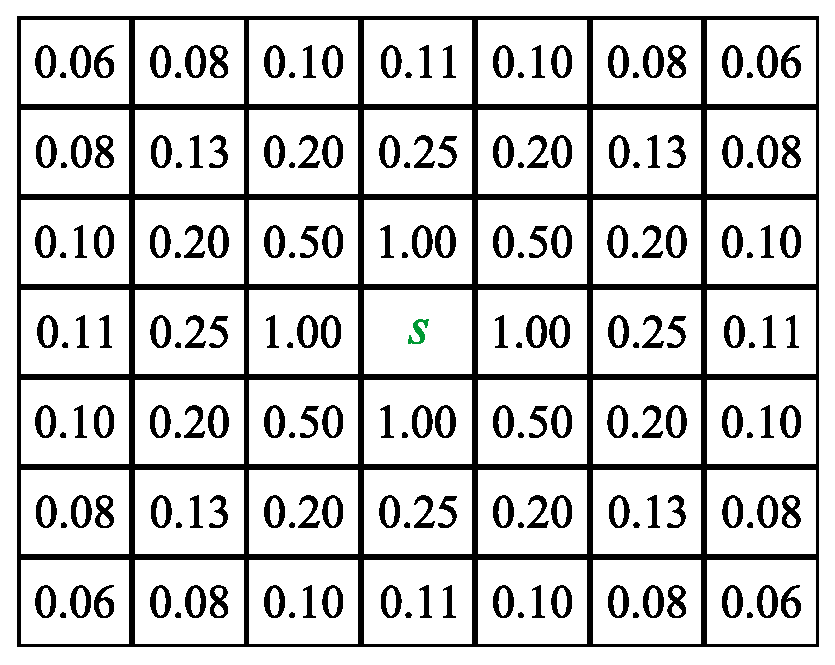
\includegraphics[width=0.4\textwidth]{distweights}
  }}
\end{picture}
%%
\begin{picture}(190,105)
  \footnotesize{
    \put(0,0){\makebox(190,105){
      %GNUPLOT: LaTeX picture with Postscript
      \begin{picture}(0,0)%
      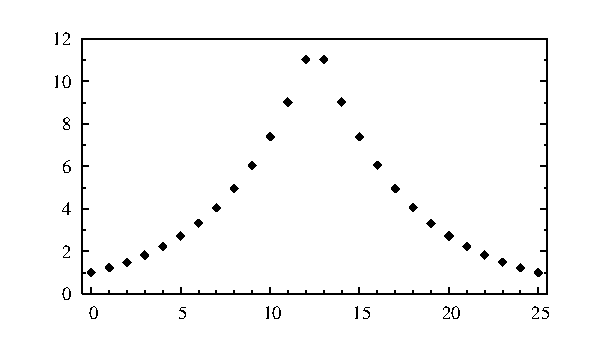
\includegraphics{posweights}%
      \end{picture}%
      \begingroup
      \setlength{\unitlength}{0.0200bp}%
      \begin{picture}(9900,5940)(0,0)%
      \put(1250,1000){\makebox(0,0)[r]{\strut{} 0}}%
      \put(1250,1740){\makebox(0,0)[r]{\strut{} 2}}%
      \put(1250,2480){\makebox(0,0)[r]{\strut{} 4}}%
      \put(1250,3220){\makebox(0,0)[r]{\strut{} 6}}%
      \put(1250,3960){\makebox(0,0)[r]{\strut{} 8}}%
      \put(1250,4700){\makebox(0,0)[r]{\strut{} 10}}%
      \put(1250,5440){\makebox(0,0)[r]{\strut{} 12}}%
      \put(1647,500){\makebox(0,0){\strut{} 0}}%
      \put(3118,500){\makebox(0,0){\strut{} 5}}%
      \put(4589,500){\makebox(0,0){\strut{} 10}}%
      \put(6061,500){\makebox(0,0){\strut{} 15}}%
      \put(7532,500){\makebox(0,0){\strut{} 20}}%
      \put(9003,500){\makebox(0,0){\strut{} 25}}%
      \end{picture}%
      \endgroup
    }}
  }
\end{picture}
%%
\vspace*{-3ex}
\caption{\label{fig:conflictindex}
  Ranges of values for both $\gamma$ and $\omega$ on a typical Affymetrix
  chip where probes of length~25 are synthesized in~74 masking steps. Left:
  approximate values of the distance-dependent weighting function
  $\gamma(s,s')$ for a spot $s$ in the center and close
  neighbors~$s'$. Right:
  position-dependent weights $\omega(\eps,t)$ on the y-axis for each value
  of~$b_{\eps,t}\in\{0,\dots,25\}$ on the x-axis, assuming $\ell_\eps=25$.}%
\end{figure}


The conflict index $\mathcal{C}(s)$ can be interpreted as the fraction of
probes in $s$ damaged because of unwanted illumination.


\section{Conflict Index and Border Length as Chip Quality Measures}
\label{sec:mlp_bl_vs_ci}

The relation between conflict index and border length becomes clear if
$\gamma(s,s')$ and $\omega(\eps,t)$ are re-defined as follows: Set
$\gamma(s,s') := 1$ if $s'$ is a direct neighbor of~$s$, and $:=0$ otherwise.
Also, set $\omega(\eps,t) := 1/2$, so that conflicts always have the same
weight, independently of where they occur. Now $\sum_s\, \mathcal{C}(s) =
\sum_{t=1}^T\, \mathcal{B}_t$; that is, total border length is equivalent to
the sum of conflict indices for a particular choice of $\gamma$ and $\omega$.
For the choices (\ref{eq:dist_weight}) and~(\ref{eq:pos_mult}), they are not
equivalent but still correlated, since a good layout has low border lengths as
well as low conflict indices.

To better compare border lengths for chips of different sizes, we
divide by the number of probes and call $1/|\mathcal{P}| \cdot
\sum_{t=1}^T\, \mathcal{B}_t$ the \emph{normalized border length};
this can be further divided by the number of synthesis steps to give
the \emph{normalized border length per mask} $1/(|\mathcal{P}|\cdot
|\mathcal{T}|) \cdot \sum_{t=1}^T\, \mathcal{B}_t$. Reasonable values
encountered in practice are between 30 and 40 per probe, or around 0.5
per probe and mask.

Similarly, we define the \emph{average conflict index} as
$1/|\mathcal{P}| \cdot \sum_s\, \mathcal{C}(s)$. The scale depends on
our choice of $\gamma$ and $\omega$. In our experiments, reasonable
values range from 300 to 600 per probe (or 4 to 8 per probe and mask).


\section{How hard is the Microarray Layout Problem?}
\label{sec:mlp_how_hard}

The MLP appears to be hard because of the super-exponential number of possible
arrangements, although no NP-hardness proof is yet known. A formulation of the
MLP as a Quadratic Assignment Problem (QAP) was given by
\citet{Carvalho2006a}.  The QAP is a classical combinatorial optimization
problem that is, in general, NP-hard, and particularly hard to solve in
practice \citep{Cela1997}. Optimal solutions are thus unlikely to be found
even for small chips and even if we assume that all probes have a single
predefined embedding.

If we consider all possible embeddings (up to several million for a typical
Affymetrix probe), the MLP is even harder. For this reason, the problem has
been traditionally tackled in two phases. First, an initial embedding of the
probes is fixed and an arrangement of these embeddings on the chip with minimum
conflicts is sought. This is usually referred to as the \emph{placement} phase.
Second, a post-placement optimization phase \emph{re-embeds} the probes
considering their location on the chip, in such a way that the conflicts with
neighboring spots are further reduced. Often, the chip is \emph{partitioned} 
into smaller sub-regions before the placement phase in order
to reduce running times, especially on larger chips.


The next chapter surveys the most important placement algorithms. Re-embedding
algorithms are then discussed in Chapter X, and partitioning
algorithms are the focus of Chapter Y. Finally, we present 
recent developments that simultaneously place and embed probes in Chapter W

